% !TEX root = ../ausarbeitung.tex

\chapter{Anforderungsanalyse und Spezifikation}

Während der Konzeption des Projekts ist klar geworden, dass die zu entwickelnde Software eine relativ komplexe Architektur erfordert. Da eine Browser Applikation entwickelt wurde, musste die Software in Teilprojekte untergliedert werden. Zum einen das User-Interface für die Web Applikation und zum Anderen die Programmlogik, welche aufgrund der benötigten Funktionalitäten (wie Datenbankanbindung und Algorithmen zur Textverarbeitung) nicht sinnvoll im Web Client implementiert werden konnte.\\
Um eine Spezifikation für die Software zu entwerfen und den zu verwendenden Software-Stack zu definieren, wurde zunächst im Gespräch mit Experten (Lerntherapeuten) eine Anforderungsanalyse durchgeführt, die im Folgendem Teil beschrieben wird. Im darauffolgenden Kapitel gehe ich Schritt für Schritt auf die Entwicklung des Gesamtsystems ein.

\section{Anforderungen an die Software}

Zunächst wurde festgestellt, welche Funktionen die Applikation dem Nutzer bieten soll. Dazu wurden folgende mögliche Szenarien aufgestellt:

\paragraph{Text Analyse} 
Die Nutzerin oder der Nutzer möchte einen Fließtext eingeben und von der Anwendung annotieren lassen. Nach der Eingabe soll das Ergebnis annotiert in der App dargestellt werden.

\paragraph{Anpassung der annotierten Darstellung}
Die Nutzerin oder der Nutzer möchte die Parameter des annotierten Texts ändern. Angepasst werden können sollen die Texteigenschaften (Font, Zeilenabstand, Zeichenabstand) und die Darstellung der Annotation (Farben für betonte und unbetonte Silbe, Silbenabstand, Trennzeichen zwischen Silben)

\paragraph{Export der annotierten Darstellung}
Die Nutzerin oder der Nutzer hat die Möglichkeit verschiedene Formate des annotierten Texts zu exportieren, z.B. Druck, HTML oder Word.

\paragraph{Verwaltung von User Accounts}
Der Nutzerin oder dem Nutzer soll die Möglichkeit gegeben werden, ein Nutzerkonto zu erstellen um persönlich verwendete Daten (z.B. Texte oder Wortsegmentierungen) speichern zu können. Dazu werden Funktionen und Interfaces zur Registrierung eines Nutzeraccounts, Login, Logout, zum Bearbeiten der Nutzerinformationen und zum Löschen des Accounts bereitgestellt.

\paragraph{Behandlung unbekannter Wörter}
Die Nutzerin oder der Nutzer kann nacheinander die Segmentierung von Wörtern, die durch das System nicht eindeutig bestimmt wurden konnten, selbst manuell festlegen.

\paragraph{Bestimmung der Segmentierung unbekannter Wörter}
Für ein unbekanntes Wort wählt der User in einem neuen View die Segmentierung selbst aus. Dafür werden folgende Möglichkeiten gegeben:
\begin{itemize}
	\item Input aus G2P Systemen wie MARY TTS
	\item Manuelle Segmentierung mit geeignetem User Interface
	\item Eventuell weitere Quellen für die Segmentierung (z.B. Duden)
\end{itemize}

\paragraph{Speicherung von Nutzer Segmentierungen}
Von der Nutzerin oder dem Nutzer hinzugefügte Segmentierungen sollen (lokal für das Nutzerkonto) gespeichert werden können und beim nächsten Vorkommen in einem Text automatisch verwendet werden.

\paragraph{Speicherung und Wiederverwendung von Annotationskonfigurationen für Texte}
Die Einstellungen, die eine Nutzerin oder ein Nutzer an einem annotierten Text vorgenommen hat, können als Vorlage für andere Texte gespeichert werden. In den Annotationseinstellungen eines Textes kann eine zuvor gespeicherte Konfiguration wiederverwendet werden.

\paragraph{Speicherung und Wiederverwendung von Nutzertexten}
Analysierte Texte können von der Nutzerin oder dem Nutzer zusammen mit der verwendeten Konfiguration gespeichert werden. Den Texten können Metadaten zugeordnet werden, z.B. Thema, Niveau, Zielgruppe. Im Benutzerbereich werden die Texte, die der Nutzer hinzugefügt hat, geeignet strukturiert, dargestellt. Es wird die Möglichkeit gegeben, den gespeicherten Text erneut analysieren zu lassen.

\paragraph{Verifizierung unbekannter Wörter}
Manuelle Segmentierungen von unbekannten Wörtern müssen auf Korrektheit überprüft werden. Dazu werden alle Nutzerinnen und Nutzer aufgefordert, die Einträge, die mit anderen Nutzerkonten erstellt wurden, zu überprüfen. In einem Fenster, ähnlich zur manuellen Segmentierung, kann die Nutzerin oder der Nutzer fremde Einträge bestätigen oder Gegenvorschläge übermitteln.

\paragraph{Expertennutzer}
Experten (z.B. LinguistInnen oder LerntherapeutInnen) können sich als solche bei der Erstellung eines Accounts identifizieren. Bei der Wort Verifizierung zählt die Stimme der ExpertennutzerInnen mehr als die von NutzerInnen, die keine ExpertInnen sind.

Hieraus lassen sich folgende grundlegende Anforderungen an die Software spezifizieren:

\begin{itemize}
	\item Service zur Textanalyse
	\item Datenbank für Wörter
	\item Service zur Manipulation der Wortdatenbank
	\item Speicherung nutzerspezifischer Daten
	\item Service zur Nutzerverwaltung
	\item Geeignetes User Interface zur Darstellung von Texten, Verwaltung der Nutzerdaten und zur Interaktion mit dem System
\end{itemize}

\subsection{User Interface}
Von den Szenarien und Anforderungen ausgehend wurde in den Folgenden Schritten ein geeignetes User Interface erarbeitet. Tabelle \ref{table:navigation} zeigt die für die Navigation wichtigsten Komponenten.

\begin{table}[h!]
	\centering
	\begin{tabular}{|l|p{8cm}|}
		\hline
		Hauptnavigationskomponente & Unterpunkte / Funktionen \\
		\hline
		\hline
		Begrüßungsseite (Home) & Informationen zum Hintergrund der Applikation und zu verfügbaren Funktionen\\
		\hline
		Textanalyse & Eingabe und Analyse von Texten, Annotation und Darstellung des Textes, sowie Funktionen zum Druck und Export\\
		\hline
		Nutzerkonto & Login, Registrierung, Verwaltung des Nutzerkontos und nutzerspezifischer Daten \\
		\hline
		Verifizierung & Verifizierung manuell segmentierter Wörter \\
		\hline
	\end{tabular}
	\caption{Hauptkomponenten der Navigationsstruktur}
	\label{table:navigation}
\end{table}

\subsubsection{Informationsstruktur}

Mithilfe dieser Überlegungen wurde festgelegt, dass es eine horizontale Navigationsleiste mit den vier aufgelisteten Hauptnavigationskomponenten geben soll. Der Link zum Nutzerkonto sollte aufgrund von Nutzergewohnheiten gesondert, rechtsbündig in der Navigationsleiste stehen (\ref{fig:navigation}). Jeder Punkt der Navigation soll Einstiegspunkt in eine Hauptkomponente der Applikation sein, es gibt keine weiteren Ebenen in der Navigationshierarchie, da die Anzahl der Komponenten überschaubar ist. Daher wird auch auf andere Navigationsmöglichkeiten, wie z.B. eine seitenweite Suche verzichtet.


\begin{figure}[h!]
	\centering
	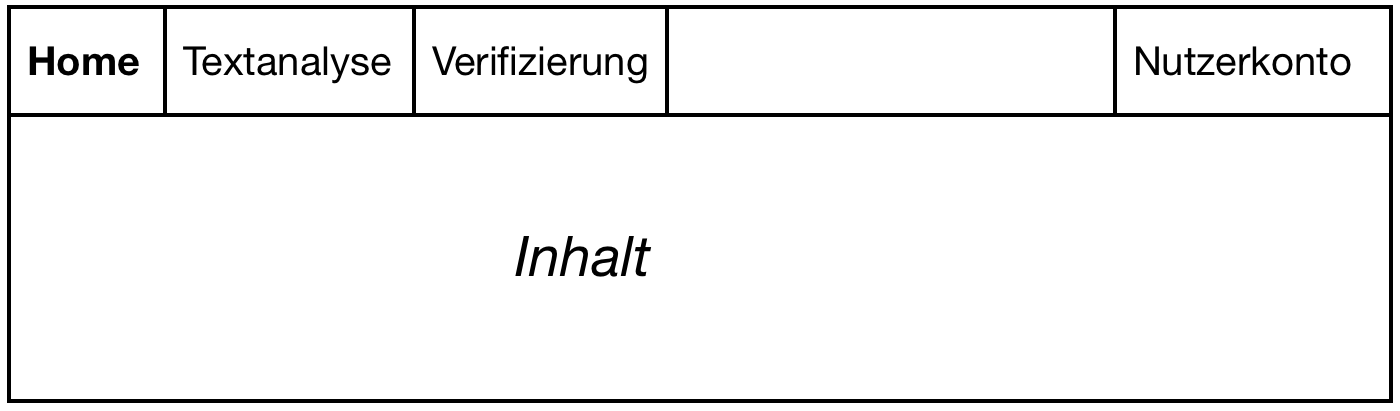
\includegraphics[width=.8\linewidth]{figures/navigation}
	\caption{Navigationsstruktur}
	\label{fig:navigation}
\end{figure}

\subsubsection{Farbschema}

Als nächstes wurde ein möglichst ansprechendes Farbschema gesucht. Hierfür wurder mit einem Farbrad (es wurde Adobe Color CC verwendet, \textit{https://color.adobe.com}) zwei Komplementärfarben als Hauptfarben ausgesucht (s. Figur \ref{fig:colors}). Die blaue Farbe wurde vor Allem für Links eingesetzt, eine hellere Version für Links im Hover Zustand. Eine weitere, ins Türkis gehende Abstufung wurde für Rahmen beim Gruppieren von Elementen auf der Seite verwendet. Der beige Farbton kommt als Hintergrundfarbe für die Navigationsleiste zum Einsatz.

\begin{figure}[h!]
	\centering
	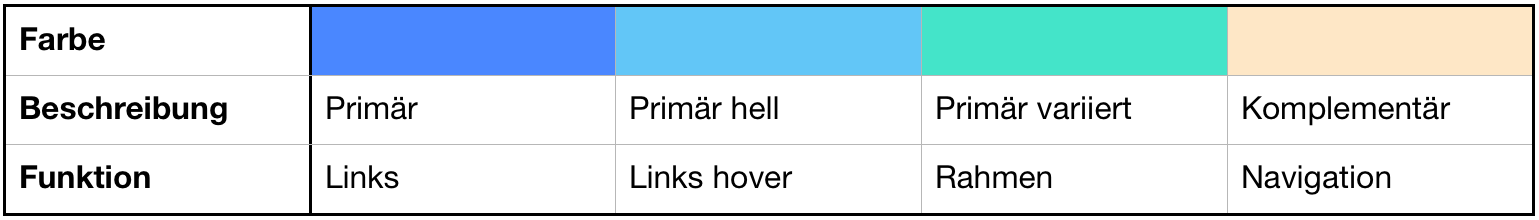
\includegraphics[width=.95\linewidth]{figures/farbschema}
	\caption{Farbschema aus Komplementärfarben}
	\label{fig:colors}
\end{figure}






\section{Softwarestack}

Bei der Vielseitigkeit der verschiedenen Anforderungen ist die Wahl der zu verwendenden Technologien nicht unerheblich. Programmiersprachen und Frameworks mussten sorgfältig ausgewählt werden um für jedes Teilproblem eine passende Lösung zu entwickeln.\\
Die erste wichtige Unterteilung fand statt, zum Einen in ein Frontend welches die Schnittstelle zum Benutzer darstellt und zum Anderen in ein Backend, welches die vom System verwendeten Daten speichert, manipuliert und diese mit Hilfe geeigneter Algorithmen an das Frontend schickt (s. Figur \ref{fig:frontendbackend}). Eine genaue Beschreibung über den Aufbau und die Funktion von Front- und Backend wird in Kapitel 4 gegeben.\\

\begin{figure}[h!]
	\centering
	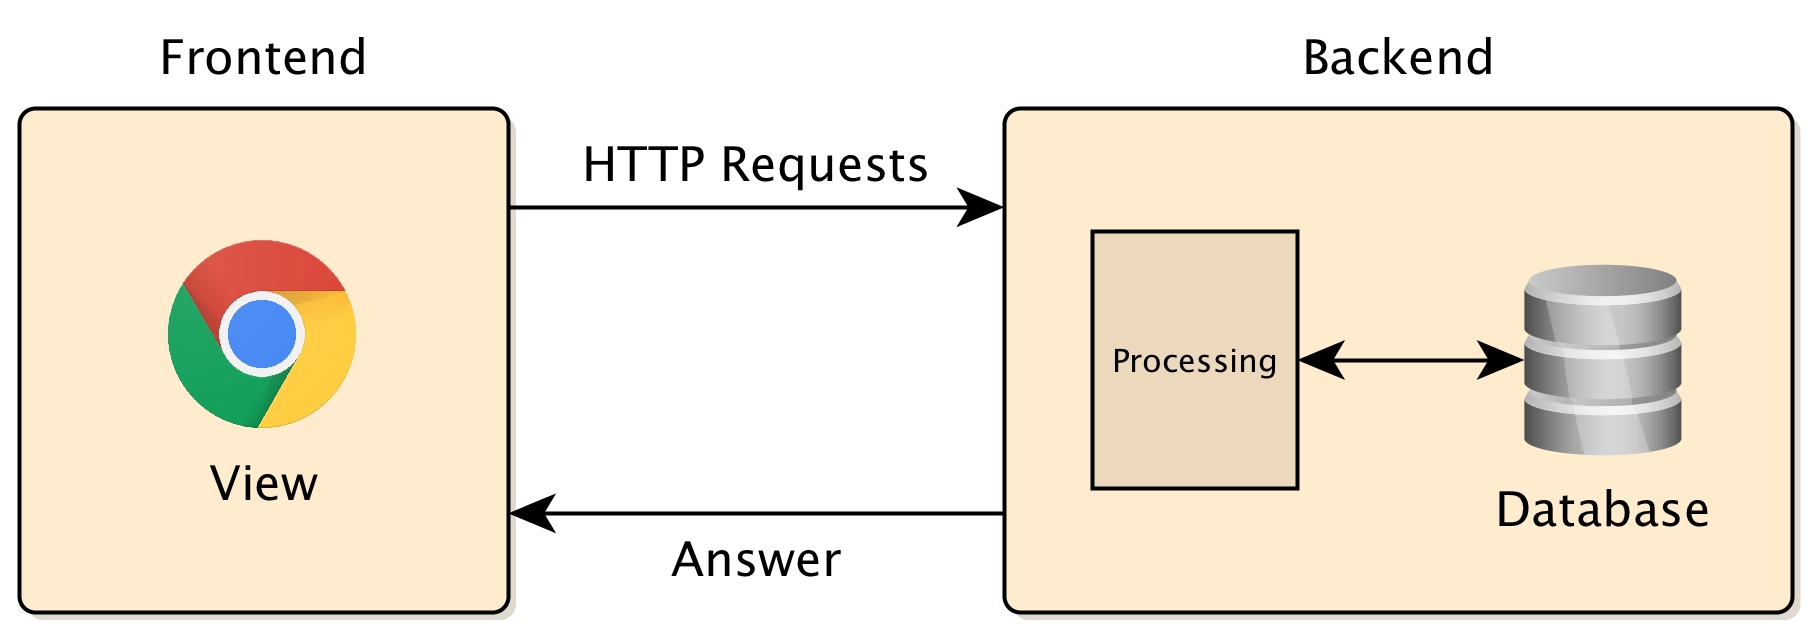
\includegraphics[width=.8\linewidth]{figures/frontendbackend}
	\caption{Kommunikation zwischen Front- und Backend}
	\label{fig:frontendbackend}
\end{figure}

Diese Aufteilung ist in der Webentwicklung weit verbreitet \tocite{front backend} und bietet einige Vorteile gegenüber eins komplett integriertem Gesamtsystems:

\begin{itemize}
	\item Klare Trennung von Darstellung und Datenverarbeitung
	\item Einfachere Fehlersuche durch kleinere Komponenten
	\item Bei der Entwickelung zusätzlicher Frontends (z.B. für Android oder iOS) muss nur ein neuer Teil des Softwaresystems entwickelt werden, während das Backend gleich bleibt.
	\item Einfache Arbeitsaufteilung im Entwicklerteam (relevant bei Weiterentwicklung der Anwendung mit mehreren Personen)
\end{itemize}

\subsection{Verwendete Technologien}
Für verschiedene zu realisierende Ziele gibt es für jedes Teilziel Technologien, die Vorteile gegenüber anderen bieten. Die Verwaltung von Datenbanken ist zum Beispiel besser mit einer serverseitigen Skriptsprache zu implementieren, als mit den Möglichkeiten, die das Frontend bietet. Im Web Frontend dagegen sind gewisse Technologien wie \textit{HTML}, \textit{CSS} und \textit{JavaScript} Standard, die zwangsläufig verwendet werden müssen. Daher wird In der Applikation eine Vielzahl verschiedener Technologien verwendet, eine Übersicht ist hier gegeben:

\begin{itemize}
	\item Backend: \textit{python}, \textit{REST}, sowie die python Frameworks fla\textit{}sk, \textit{spacy} und \textit{sqlalchemy}
	\item Frontend: \textit{HTML}, \textit{CSS}, \textit{JavaScript}, \textit{AngularDart}
	\item Kommunikation mit \textit{JSON}
	\item Deployment mit \textit{Apache} auf \textit{AWS} Server
\end{itemize}

Im Folgenden werden die einzelnen Technologien und die Gründe für deren Verwendung beschrieben.

\subsection{Backend}

Um die Entwicklung des Backends möglichst einfach zu halten, wurde zunächst untersucht, ob ein fertiges Backend (Backend as a service) verwendet werden kann. Hierzu können z.B. fertige Services wie MongoDB oder Firebase mit integrierter NoSQL Datenbank verwendet werden\cite{almootassem2017}.\\
Zunächst wurde Firebase genauer untersucht und testweise implementiert. Prinzipiell war es gut möglich, eine Verbindung mit dem Frontend herzustellen (Daten in der Firebase Datenbank können mit HTTP Requests geschrieben und gelesen werden). Die Möglichkeiten des Backends beschränkten sich allerdings auf Datenmanipulation und Cloud Code (serverseitiges JavaScript in Firebase).\\
Ein Problem dabei war, dass komplexere Logik wie das \textit{Natural Language Processing} nur entweder im Frontend oder im Backend mit \textit{JavaScript} implementiert werden konnte. NLP frameworks, wie es sie z.B. in \textit{python} oder \textit{Java} gibt, konnten somit nicht verwendet werden. Wurde der Text im Frontend in einzelne Wörter zerlegt und diese in der Firebase Datenbank nachgeschlagen, musste zudem für jedes Wort ein HTTP Request geschickt werden, was zu unbefriedigenden Antwortzeiten führte.\\

Aufgrund der beschriebenen Probleme wurde parallel ein alternatives Backend in python implementiert. Die Entwicklung der Softwarearchitektur wurde an den Representational State Transfer (REST) angelehnt. Dieser beschreibt Prinzipien und Restriktionen für die Konzeption von Webarchitekturen\cite{Fielding:2000:ASD:932295}. Diese Lösung brachte zwar wiederum eigene Schwierigkeiten und Probleme mit sich (s. Abschnitt \ref{sec:deployment}), wurde aber später für die einfachere und schneller zu entwickelnde Variante erachtet und daher weiter verfolgt. Da in der Praxis die Entwicklung und Wartung eines eigenen Backends einen erheblichen Mehraufwand bedeuten kann, wäre weiterführend auch eine kombinierte Lösung denkbar, in der ein Backend-as-a-Service wie Firebase benutzt wird, aber zwischen Front- und Backend noch eine weitere Schicht installiert wird, welche Programm Logik enthält und NLP Berechnungen durchführt.\\

Die Einhaltung der REST Restriktionen (z.B. muss das Backend zustandslos sein und die Anfragen resourcenorientiert formuliert werden) wurden so gut es im Rahmen der Arbeit möglich war eingehalten, allerdings konnte die Entwicklung einer konsequenten Softwarearchitektur nicht im Vordergrund stehen, da die entwickelte Applikation lediglich als Prototyp betrachtet werden muss.\\

\subsubsection{Python}
\label{sec:python}

Die Verwendung von \textit{Python}\cite{vanRossum2011} im Backend brachte einige Vorteile für die Effizienz sowie für eine gute Strukturierung des Projekts, da ein großer Teil der Programmlogik im Backend abgebildet und somit die Komplexität des Frontends entlastet werden konnte. Zudem konnten nützliche Frameworks für NLP oder für die Verarbeitung der HTTP Requests benutzt werden.

\subsubsection{Flask}
\label{sec:flask}

\textit{Flask} ist ein \textit{python} Framework für die Webentwicklung. Es kann z.B. eingesetzt werden, um Webseiten an Clients auszuliefern, allerdings auch um eine API zu entwickeln, welche nur Daten an einen Client schickt anstatt ganzer Webseiten. Bei der Entwicklung einer Flask Applikation wird zunächst im Python Skript ein Applikationsobjekt angelegt. Die Applikation kann in Python konfiguriert und mit einem Funktionsaufruf gestartet werden.\\
Alle beim Server ankommenden HTTP Requests werden von \textit{Flask} automatisch verarbeitet. Das Verhalten für eigene Routen kann durch annotierte Funktionsdefinitionen angepasst werden. Figur \ref{fig:flask} zeigt ein Beispiel, wie das Erstellen einer Resource mit einem HTTP Request an eine selbst definierte Methode weitergeleitet wird.

\begin{figure}
	\begin{lstlisting}
@app.route('/user/word/add', methods=['POST'])
def user_add_word():
...
	\end{lstlisting}
	\caption{Definition von \textit{Flask} Routen}
	\label{fig:flask}
\end{figure}

\subsubsection{spacy}
\label{sec:spacy}
parser, alternative NLTK, auch benutzt, warum ist spacy besser?\\
\todo{quelle, dass spacy der performanteste parser ist}
tokenizer, part of speech

\subsection{Frontend}

webapplication, html css, single-view-application, dynamic data loading
viele frameworks, verwende AngularDart
no javascript: weakly typed languages transforming to JS: GWT (java), typescript, Dart

\subsubsection{Angular Dart}
\label{sec:angulardart}
warum? javascript is bad.\\

data binding\\
more lightweight vs Java\\

many google apps use it\\
objektorientierung\\

angular? angular2?\\

dart, google\\
alternativen, typescript...\\

dart2js compiler, wie funktioniert dieser\\

\subsection{Deployment}
\label{sec:deployment}
webserver für frontend, auf eigenem server mit apache gehostet\\
flask python service läuft immer, REST schnittstelle\\
\todo{vernachlässigung von security}





%-----------------------------------------------------------------------------------------
%-----------------------------------------------------------------------------------------
